\section{Quality Assurance}
\label{sec:fdsp-tpcelec-qa}

The \dword{tpc} electronics consortium is developing a \dword{qa} plan consistent
with the principles discussed in \tcchqa.
The goal of the \dword{qa} plan is to maximize the number of functioning
readout channels in the detector that achieve the performance specifications
for the detector discussed in Section~\ref{sec:fdsp-tpcelec-overview-design},
particularly on noise. Minimizing the noise levels in the detector requires that all
system aspects are considered starting from the design phase, and in this
respect, the experience gained with the \dword{pdsp} prototype is extremely
valuable as it informs necessary design changes in the detector 
components. The lessons learned during the construction of \dword{pdsp},
the commissioning of the detector, and the initial data taking period have
already been discussed in Section~\ref{sec:fdsp-tpcelec-design}. Further
operation of \dword{pdsp} in 2019 has provided information on the
long term stability of the detector components.

Apart from the number of channels, the most important difference
between \dword{pdsp} and \dword{dune} is the projected lifetime of the detector. This
is relevant because a significant fraction of the detector components provided 
by the \dword{tpc} electronics consortium are installed inside the cryostat and cannot 
be accessed or repaired during the operational lifetime of the detector. The 
graded approach to \dword{qa} indicates that particular care must be used for
the \dword{ce} components that will be installed inside the cryostat.

A complete \dword{qa} plan starts with ensuring that the designs of all
detector components fulfill the specification criteria, considering
also system aspects, i.e. how the various detector components interact
among themselves and with the detector components provided by other 
consortia. We discuss validating the design in 
Section~\ref{sec:fdsp-tpcelec-qa-initial} and the facilities that we use
to investigate the interactions among different detector components
in Section~\ref{sec:fdsp-tpcelec-qa-facilities}. 

The other aspects of the \dword{qa} plan involve documenting the 
assembly and testing processes, storing and analyzing the information
collected during the \dword{qc} process, training and qualifying 
personnel from the consortium, monitoring procurement of 
components from external vendors, and assessing whether the
\dword{qc} procedures are applied uniformly across
the various sites involved in detector construction, integration,
and installation. The \dword{tpc} electronics consortium plan involves
having multiple sites using the same \dword{qc} procedures,
many of which will be developed as part of system design tests during the \dword{qa} phase,
with the possibility of a significant turnover in the personnel
performing these tasks. To avoid problems during most of the
production phase, we plan to emphasize training as well as documentation
of the \dword{qa} plan. Reference parts will be tested at
several sites to ensure consistent results. At
a single site, some parts will be tested repeatedly to ensure
that the response of the apparatus does not change and
that new personnel involved in testing detector components are 
as proficient as more experienced personnel. 

All data from
the \dword{qc} process will be stored in a common database, and
the yields of the production will be centrally monitored and 
compared among different sites. The procedures adopted
for detector construction will evolve from the experience
gained with \dword{pdsp}. A first version of the testing procedures
will be put in place in 2019 and 2020, while the final designs of
the detector components are completed and new prototypes are
tested. The \dword{qc} procedures will then be reviewed
during the engineering design review that precedes pre-production. Lessons learned during pre-production
will be analyzed, and a final and improved \dword{qc} process will be 
developed before the production readiness review that triggers
the beginning of production. During production, the results
of the \dword{qc} process will be reviewed at regular intervals
in production progress reviews. In case of problems, production
will be stopped and the problematic issues assessed, 
followed by changes in the procedures if necessary.

%%%%%%%%%%%%%%%%%%%%%%%%%%%%%%%%%%%
\subsection{Initial Design Validation}
\label{sec:fdsp-tpcelec-qa-initial}

As described in Section~\ref{sec:fdsp-tpcelec-design}, four \dword{asic} designs
are being developed for the \dword{dune} \dword{fd} single-phase \dword{tpc} readout 
(\dword{larasic}, \dword{coldadc}, \dword{coldata}, and \dword{cryo}). 
When a new prototype \dword{asic} is produced, the groups responsible for the \dword{asic} design will perform the first tests of 
\dword{asic} functionality and performance. These tests may use either 
packaged parts or dice mounted directly on a printed circuit board 
and wire bonded to the board.  The goal of these tests is to determine 
the extent to which the \dword{asic} functions as intended, both at room 
temperature and at \lntwo temperature.  For all chips, these tests 
include exercising digital control logic and all modes of operation. Tests 
of \dword{fe} \dwords{asic} include measurements of noise levels as a function 
of input capacitance, baseline recovery from large pulses, cross-talk, linearity, 
and dynamic range. Tests of \dwords{adc} include measurements of the effective noise levels and 
of differential as well as integral non-linearity. Tests of the \dword{coldata} and \dword{cryo} \dwords{asic}
include verification of both the control and high-speed data output links using 
cables with lengths of \SI{9}{m} and \SI{22}{m} as required for the \dword{dune} \dword{fd}.
After the initial functionality
tests by the groups that designed the \dwords{asic}, further
tests will be performed by other independent groups; then the \dwords{asic}
will be mounted on \dwords{femb} so noise measurements can be repeated
with real \dword{apa}s attached to the readout chain.

Tests of \dwords{asic} and \dwords{femb} in a cryogenic environment
are performed in \lntwo instead of \dword{lar} for cost reasons, ignoring
the small temperature difference. These tests can be performed immersing
the detector components in a dewar containing \lntwo for the duration
of the tests. Condensation of water from air can interfere with
the tests or damage the detector components or the test equipment,
particularly during their extraction from the \lntwo. A test dewar
design developed by Michigan State University, referred to as the
\dword{cts}, has been developed to avoid
this problem and to automate the immersion and the retrieval of 
the components being tested. Several \dword{cts} units
were deployed at \dword{bnl} during the \dword{pdsp} construction
and used for the \dword{qc} on the \dwords{asic} and \dwords{femb}
for \dword{pdsp}. Later they were also used to perform similar tasks
during the construction of the electronics for \dword{sbnd}.
Several other \dword{cts} units have been deployed to institutions involved in
developing \dwords{asic} to test the first prototypes of \dwords{asic}
and \dwords{femb} for the \dword{dune} \dword{fd}. Two \dword{cts} units 
in operation at \dword{bnl} are shown in Figure~\ref{fig:CTS}.

\begin{dunefigure}
[The Cryogenic Test System]
{fig:CTS}
{Cryogenic Test System (CTS): an insulated box is mounted on top of a commercial \lntwo dewar.  Simple controls allow the box to be purged with nitrogen gas and \lntwo to be moved from the dewar to the box and back to the dewar.}
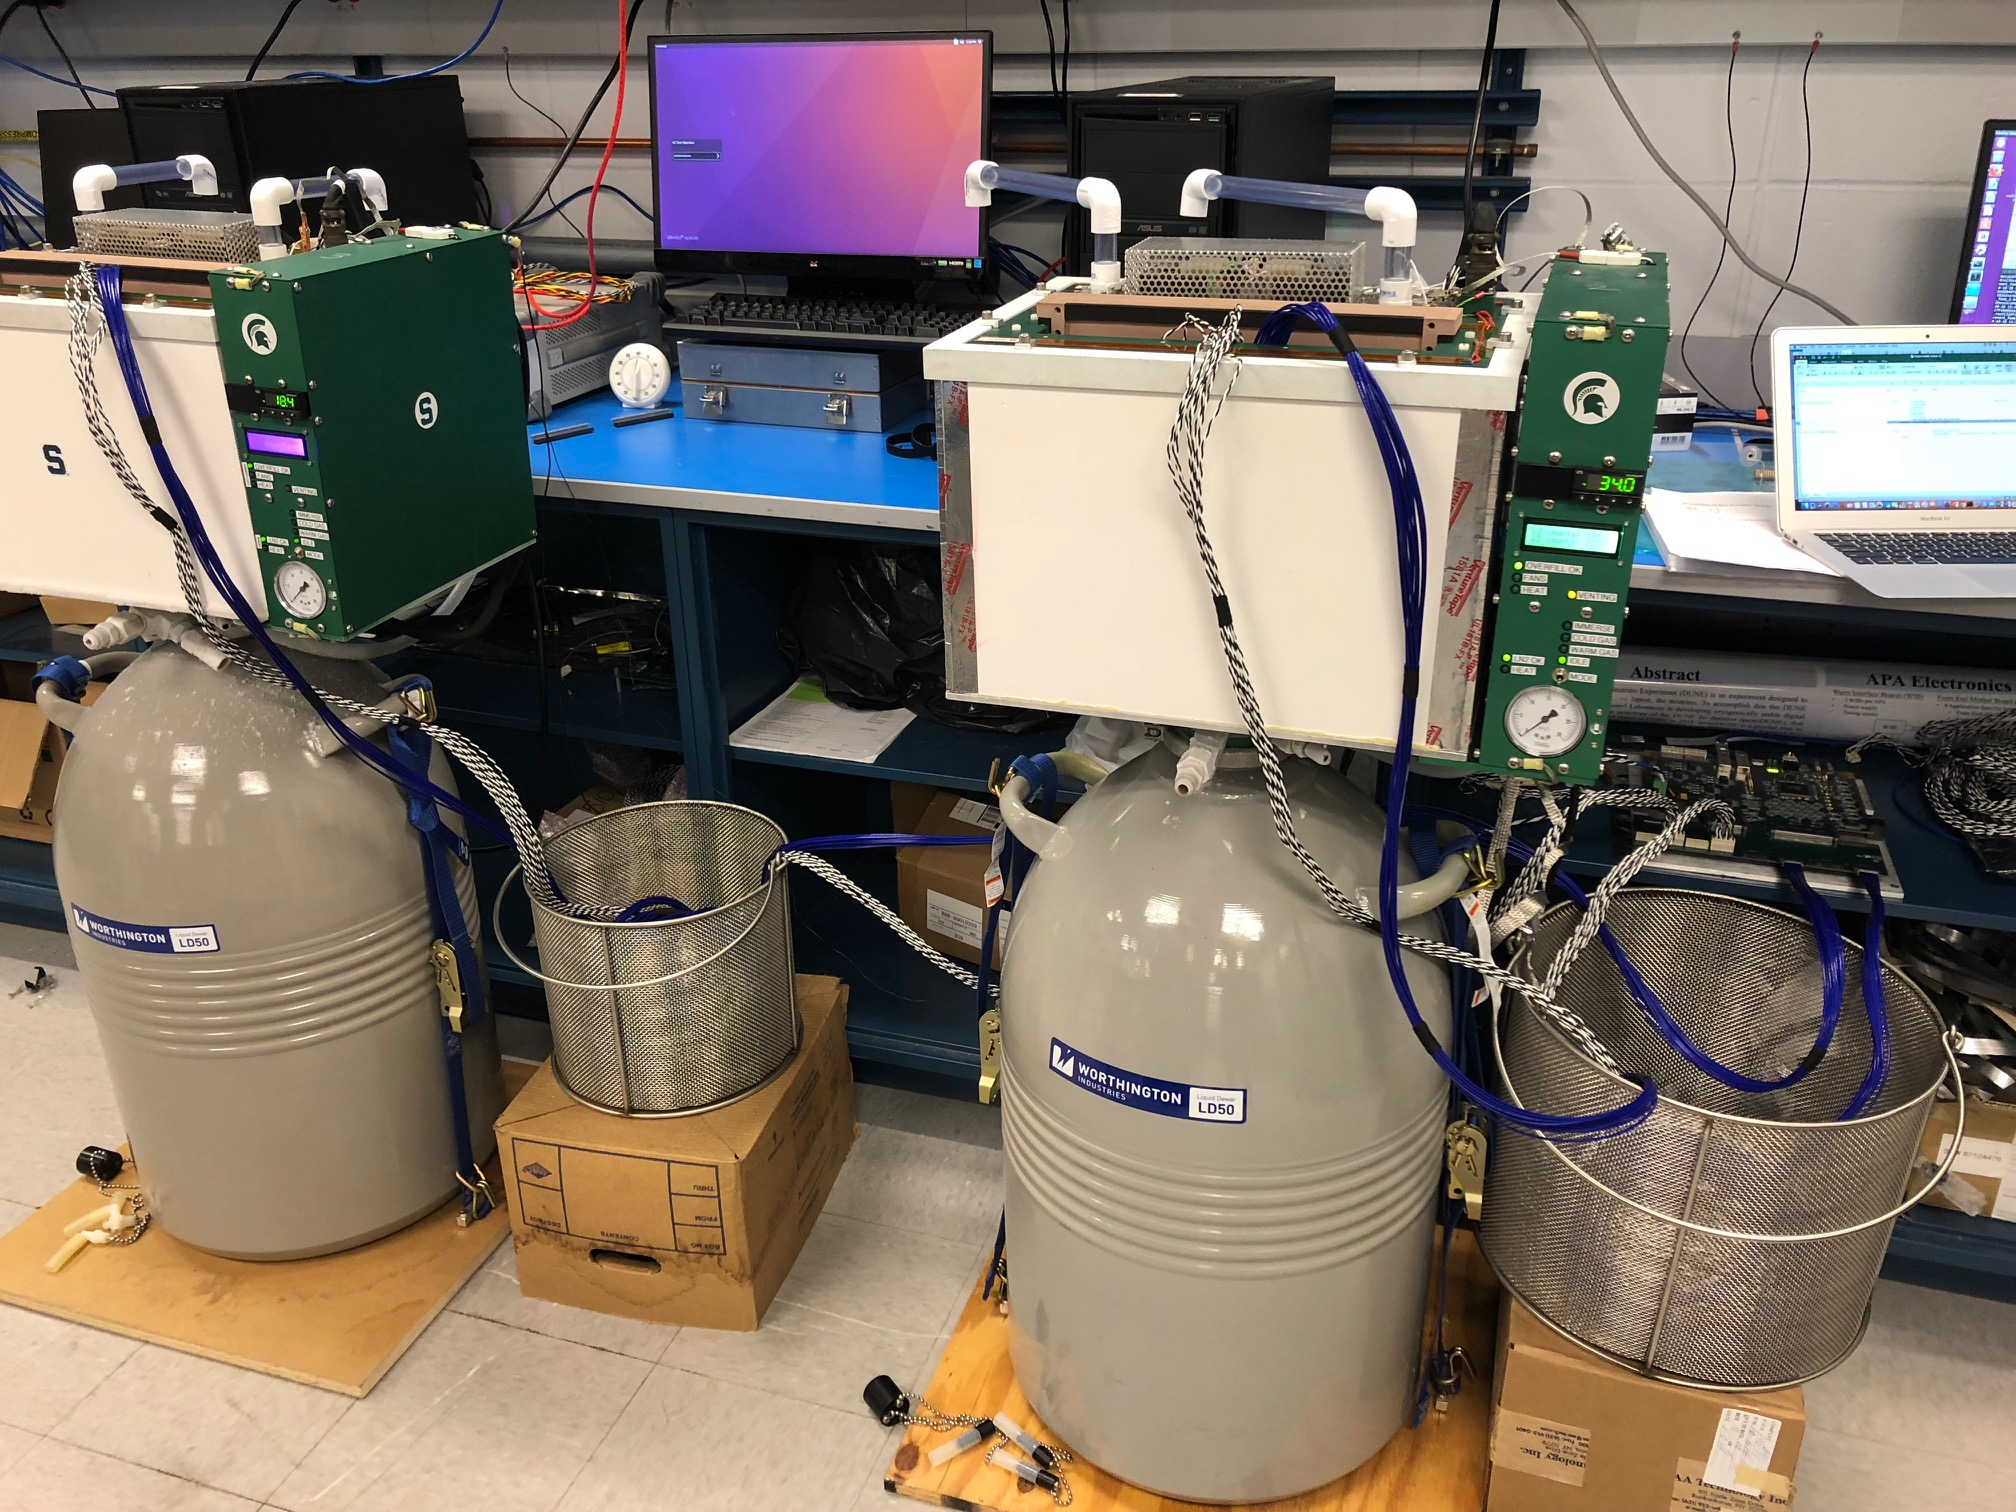
\includegraphics[width=0.4\linewidth]{sp-tpcelec-CTS2.jpeg}
\end{dunefigure}


%%%%%%%%%%%%%%%%%%%%%%%%%%%%%%%%%%%
\subsection{Integrated Test Facilities}
\label{sec:fdsp-tpcelec-qa-facilities}

The investigation of the system issues that can arise from the interaction 
of different detector components requires that a full system test of a slice
of the entire detector is performed. These tests are performed with \dwords{femb}
attached to \dword{apa}s enclosed in a structure that provides the same
grounding environment planned for the final \dword{dune} \dword{fd}. 
Power, control, and signal readout connections will be provided using cryostat 
penetrations similar to those planned for use in the \dword{dune} \dword{fd}.
Prototypes of the final \dword{dune} \dword{fd} \dword{daq} will be used for readout and
control of the detector, and if possible the \dword{pds} will also be included.
We have identified three such system test stands
that we can use for system tests: the \dword{pdsp} facility at CERN, the
\dword{iceberg} facility at \dword{fnal}, and the \num{40}\,\% \dword{apa} at \dword{bnl}.
We discuss these three setups in this section.

%%%%%%%%%%%%%%%%%%
\subsubsection{ProtoDUNE-SP and Cold Box at CERN}
\label{sec:fdsp-tpcelec-qa-facilities-pdune}

\dword{pdsp} is designed as a full slice of the \dword{dune} \dword{spmod}  
using components with a design as close as possible to the one that will
be used in production. It contains six full-size 
\dword{dune} \dword{apa}s instrumented with \num{20} \dwords{femb} each for a 
total readout channel count of \num{15360} digitized sense wires. Critically, 
the wires on each \dword{apa} are read out via a full \dword{tpc} electronics readout 
system, including a \dword{ce} flange and \dword{wiec} with five \dwords{wib} 
and one \dword{ptc}. Each combined \dword{apa} and \dword{ce} readout unit follows 
the grounding guidelines described in Section~\ref{sec:fdsp-tpcelec-design-grounding} 
to operate in a fully-isolated way with respect to the rest of the detector.

\dword{pdsp} took beam data in the CERN Neutrino Platform in 2018 and will continue
to take cosmic data throughout 2019. As described in Section~\ref{sec:fdsp-tpcelec-overview-pdune},
the live channel count (99.7\%) and average noise levels on the collection and induction wires 
(ENC~$\sim$\SI{550}{e$^-$} and $\sim$\SI{650}{e$^-$}, respectively) satisfy the \dword{dune}-\dword{sp} requirements described 
in Section~\ref{sec:fdsp-tpcelec-overview-requirements}. Several lessons learned from the production 
and testing of the \dword{tpc} electronics and the \dword{pdsp} beam data run will be incorporated into the 
next iteration of the system design for the \dword{dune} \dword{spmod}, as discussed in 
Section~\ref{sec:fdsp-tpcelec-overview-lessons}.

Five of the six \dword{apa}s were tested in the \dword{pdsp} cold box
before they were installed in the cryostat. These tests were critical
in identifying issues with \dword{ce} components after installation
on the \dword{apa}. Therefore, a very similar set of cold box tests are planned at \dword{surf} 
with the fully-instrumented \dword{dune} \dword{apa}s. A seventh \dword{apa} was delivered
to CERN in March 2019 and will be first equipped with \dword{pdsp} \dwords{femb}. This
\dword{apa} was characterized in October 2019 in the cold box like the \dword{apa}s installed
in \dword{pdsp}, establishing a reference point for further tests that will be
performed after replacing half of the \dwords{femb} with new prototypes \dwords{femb} (equipped with prototypes of the
new \dword{asic} designs). Tests will be performed in 
winter 2019 using \dwords{femb} equipped with the \dword{cots} \dword{adc}, \dwords{femb}
with the \dword{cryo} \dword{asic}, and \dwords{femb} with the new \dword{coldadc} and
\dword{coldata} \dwords{asic}. The cold box will also be used to study the effect of
low temperature on the low-voltage power and bias-voltage power cables as they are 
routed through the \dword{apa} frame.

The \dword{dune} \dword{apa}s and the readout electronics will differ from the ones used 
in \dword{pdsp}. For this reason, we are planning to re-open the \dword{pdsp} cryostat 
and replace three of the six \dword{apa}s with final \dword{dune} \dword{fd} prototypes that also include 
the most recent prototypes of the \dwords{femb} built using the chosen \dword{asic} solution.
If possible, \dwords{asic} from the engineering 
run will be used to populate the \dwords{femb} instead of using prototypes from a multi-purpose
wafer fabrication run. A total of \num{60} \dwords{femb} are required to populate the three 
final \dword{dune} \dword{apa} prototypes to be installed in \dword{pdsp}. A second period of data taking 
with this new configuration of \dword{pdsp} is planned for 2021-2022. This will also 
allow another opportunity to check for interference between the readout of the \dword{apa} 
wires and the \dword{pds} or other cryogenic instrumentation. 

%%%%%%%%%%%%%%%%%%
\subsubsection{Small Test TPC (ICEBERG)}
\label{sec:fdsp-tpcelec-qa-facilities-testtpc}

While the cold box test at CERN and \dword{pdsp} operations provide important 
validation of the \dword{tpc} electronics for DUNE, a new cryostat (\dword{iceberg}) 
has been built to test multiple \dword{ce} prototypes in a \dword{lartpc} environment.
\dword{iceberg} will be used for 
\dword{lar} detector R\&D and for system tests of the \dword{ce} prototypes. 
The \dword{iceberg} cryostat allows for rapid turn-around in testing new configurations
of the \dword{ce}. One cycle, including installing new \dwords{femb}, filling the cryostat,
performing measurements, and finally emptying the cryostat, can be completed in less than
one month. While this is slower than the turn-around that can be achieved with the
cold box at CERN, the advantage of \dword{iceberg} is that it houses a small \dword{tpc} which
allows measurements with ionization tracks, which is not possible when performing
tests in the cold box. In addition, \dword{iceberg} enables system-wide studies with new
prototypes of the \dword{pds} because the scaled-down \dword{apa} is mechanically compatible with the 
new design of the \dword{pds}, which is not the case for the seventh \dword{pdsp} \dword{apa}.  

The \dword{iceberg} cryostat, shown in Figure~\ref{fig:ICEBERG-cryotee}, is installed
at the Proton Assembly Building at \dword{fnal}. It has an inner diameter of \SI{152}{cm}
and can hold about 35,000 liters of \dword{lar}, sufficient to house a
\dword{tpc} with dimensions \SI{115}{cm}~$\times$~\SI{100}{cm}~$\times$~\SI{60}{cm}. For
\dword{dune} purposes, this cryostat will house a 1,280-channel \dword{tpc}, shown in
Figure~\ref{fig:ICEBERG-tpcdaq}, with an \dword{apa} and two \dwords{fc} that
together enclose two sensitive ionization drift volumes. Each drift volume has 
a maximum drift distance of \SI{30}{cm}. The \dword{apa} 
has been built using wire boards and anchoring elements identical to
those of \dword{pdsp}, as 
described in Section~\ref{sec:fdsp-apa-boards}. It has dimensions of 
1/10$^{\mathrm{th}}$ of a \dword{dune} \dword{apa}. The \dword{apa} mechanics are designed to
accommodate two half-length \dword{pdsp} photodetectors with dimensions and connectors that already 
include the design modifications planned for the \dword{dune} \dword{fd}.

\begin{dunefigure}
[ICEBERG cryostat and top plate spool piece]
{fig:ICEBERG-cryotee}
{\dword{iceberg} cryostat (left) and top plate spool piece (right).}
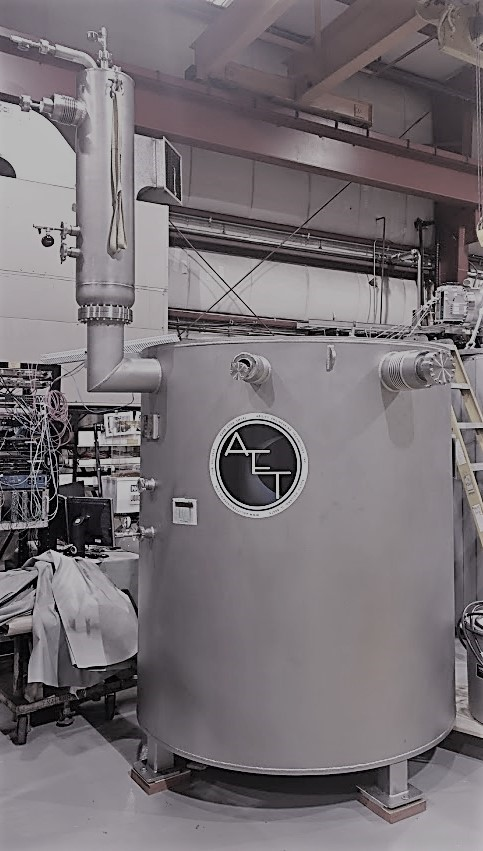
\includegraphics[width=0.26\linewidth]{sp-tpcelec-ICEBERG-cryostat.jpg}
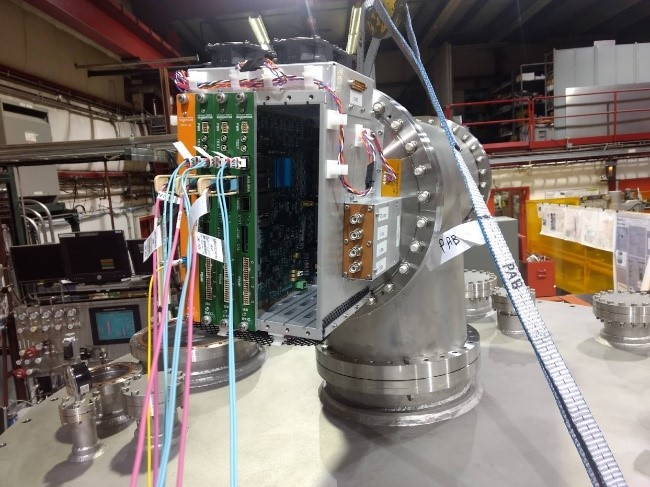
\includegraphics[width=0.61\linewidth]{sp-tpcelec-ICEBERG-Tee.jpg}
\end{dunefigure}

\begin{dunefigure}
[ICEBERG TPC and DAQ rack]
{fig:ICEBERG-tpcdaq}
{\dword{iceberg} TPC (left) and DAQ system (right).}
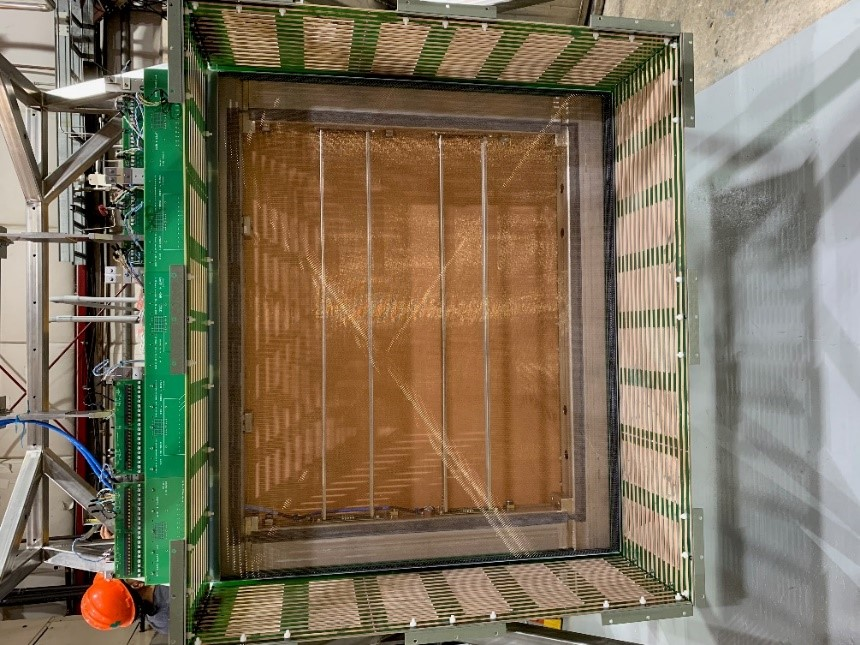
\includegraphics[angle=270,width=0.43\linewidth]{sp-tpcelec-ICEBERG-TPC.jpg}
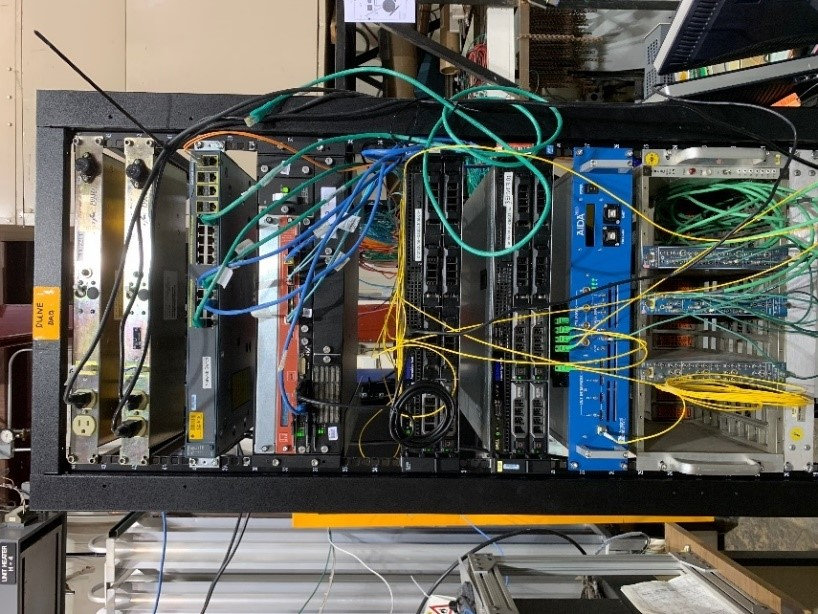
\includegraphics[angle=270,width=0.43\linewidth]{sp-tpcelec-ICEBERG-DAQ.jpg}
\end{dunefigure}

Power, readout, and controls use equipment identical to those used for \dword{pdsp}. The
interface between the \dwords{femb} and the \dword{apa} wires uses the same \dword{cr} boards
used for \dword{pdsp} and described in Section~\ref{sec:fdsp-apa-boards}. The \dword{tpc} is
read out via a \dword{daq} system (also shown in Figure~\ref{fig:ICEBERG-tpcdaq})
identical to that of \dword{pdsp}. The power and signal cables for the detector 
are routed through a spool piece installed on the center port of a movable flange on the 
top of the cryostat, which is also used to support the \dword{tpc}. The movable 
flange contains fourteen additional ports that are available for different utilities, 
including \dword{hv}, purity monitoring, cryogenic controls, and visual inspection. 
A condenser as well as \dword{lar} fill and vacuum ports are on the side of the cryostat, 
providing easy access to the detector.

The \dword{fc} for the \dword{tpc} is constructed using printed circuit boards and 
designed to provide  up to \SI{30}{cm} of drift length on both sides of the \dword{apa}. The cathode 
plane is made of a printed circuit board coated with copper and is powered with 
\SI{-15}{kV} DC power. A \SI{1}{G$\Omega$} resistance between the strips of the \dword{fc}
creates a gradient field changing from \SI{-15}{kV} at the cathode to \SI{-1}{kV} near the 
\dword{apa}. In the initial configuration, the sides of the \dwords{fc} are terminated on the \dword{apa}
ground with \SI{156}{M$\Omega$} resistors, which is different from that which has been
planned for the \dword{dune} \dword{fd}, where the last electrode of the \dwords{fc} is also connected to
a separate bias voltage supply. 

The \dword{iceberg} power system that provides power to the detector, electronics, 
\dword{daq}, and cryogenics controls was designed with extreme care to 
isolate the detector and building grounds, following the same principles adopted
for \dword{pdsp} and including a new \SI{480}{V} transformer. The impedance between the detector
and building grounds is continuously monitored. The distribution panel, which is 
at detector ground, provides both \SI{208}{V} and \SI{120}{V} lines for the \dword{tpc} electronics rack, 
providing both the low-voltage power to the \dword{tpc} electronics components and the bias 
voltage to the \dword{apa} wire planes through the \dword{wiec} and \dword{shv}
connectors located on the cryostat penetration. A single WIENER MPOD provides 
\SI{-665}{V}, \SI{-370}{V}, \SI{0}{V}, and \SI{820}{V} to the $G$, $U$, $V$, and 
$X$ planes of the \dword{apa}, respectively. It is also used to provide the 
\SI{-15}{kV} to the cathode plane. A WIENER PL506 provides the low-voltage
power to the \dword{ptc}, to the fans, and to the heaters located on the 
flange that is mounted on the spool piece at the top of the cryostat. 

The \dword{daq} for \dword{iceberg} is a copy of the system used for the readout
of five of the \dword{pdsp} \dword{apa}s at CERN. The core of the \dword{daq} system 
consists of two Linux PCs that communicate over 10 Gbps optical fibers
with processing units called \dwords{rce}, which are \dwords{fpga} that are
housed on industry-standard \dword{atca} shelves on \dword{cob} motherboards.
The \dwords{rce} can perform data compression and zero suppression. They also buffer
the data while waiting for a trigger and then send it to the Linux PCs where the data can
be analyzed using the \dword{artdaq} framework. A pair of scintillators at the top and
bottom of the cryostat generates a cosmic trigger for the \dword{daq}.
The system is modular and could be upgraded to follow the overall \dword{dune} \dword{fd} \dword{daq} 
development. 

The \dword{iceberg} cryostat was filled for the first time with \dword{lar}
in March 2018, with \dword{pdsp} \dwords{femb} installed on the \dword{tpc}. The
initial data taking run uncovered some issues with the pressure regulation system of
the cryostat and with the field cage. Once these problems were addressed, a second
data taking period started in June 2019, demonstrating stable operations of the
cryostat and \dword{tpc}. The baseline performance of the \dword{iceberg} 
\dword{tpc} has been established using \dword{pdsp} \dwords{femb}. 
As shown in Figure~\ref{fig:ENC-all-ICEBERG}, noise levels of 
$\sim\SI{300}{e^-}$ have been measured on the collection and induction wires,
which are of similar length, in line with expectations given the input capacitance
to the \dword{fe} electronics. A small number of channels have larger noise levels as a
result of the underperforming \dword{adc} electronics, as in the case of \dword{pdsp}.
\dword{tpc} noise levels remained constant while the \dword{pds} was
being operated, demonstrating that there is no interference between that system
and the \dword{tpc} electronics. Moving forward, \dword{iceberg} will be used to
test new \dword{femb} prototypes, equipped with the new \dwords{asic} under
development. 

\begin{dunefigure}
[ENC levels for all channels of the ICEBERG TPC]
{fig:ENC-all-ICEBERG}
{\dword{enc} levels (in electrons) for all channels of the \dword{iceberg} \dword{tpc},
both before and after the application of a simple offline common-mode noise filter.}
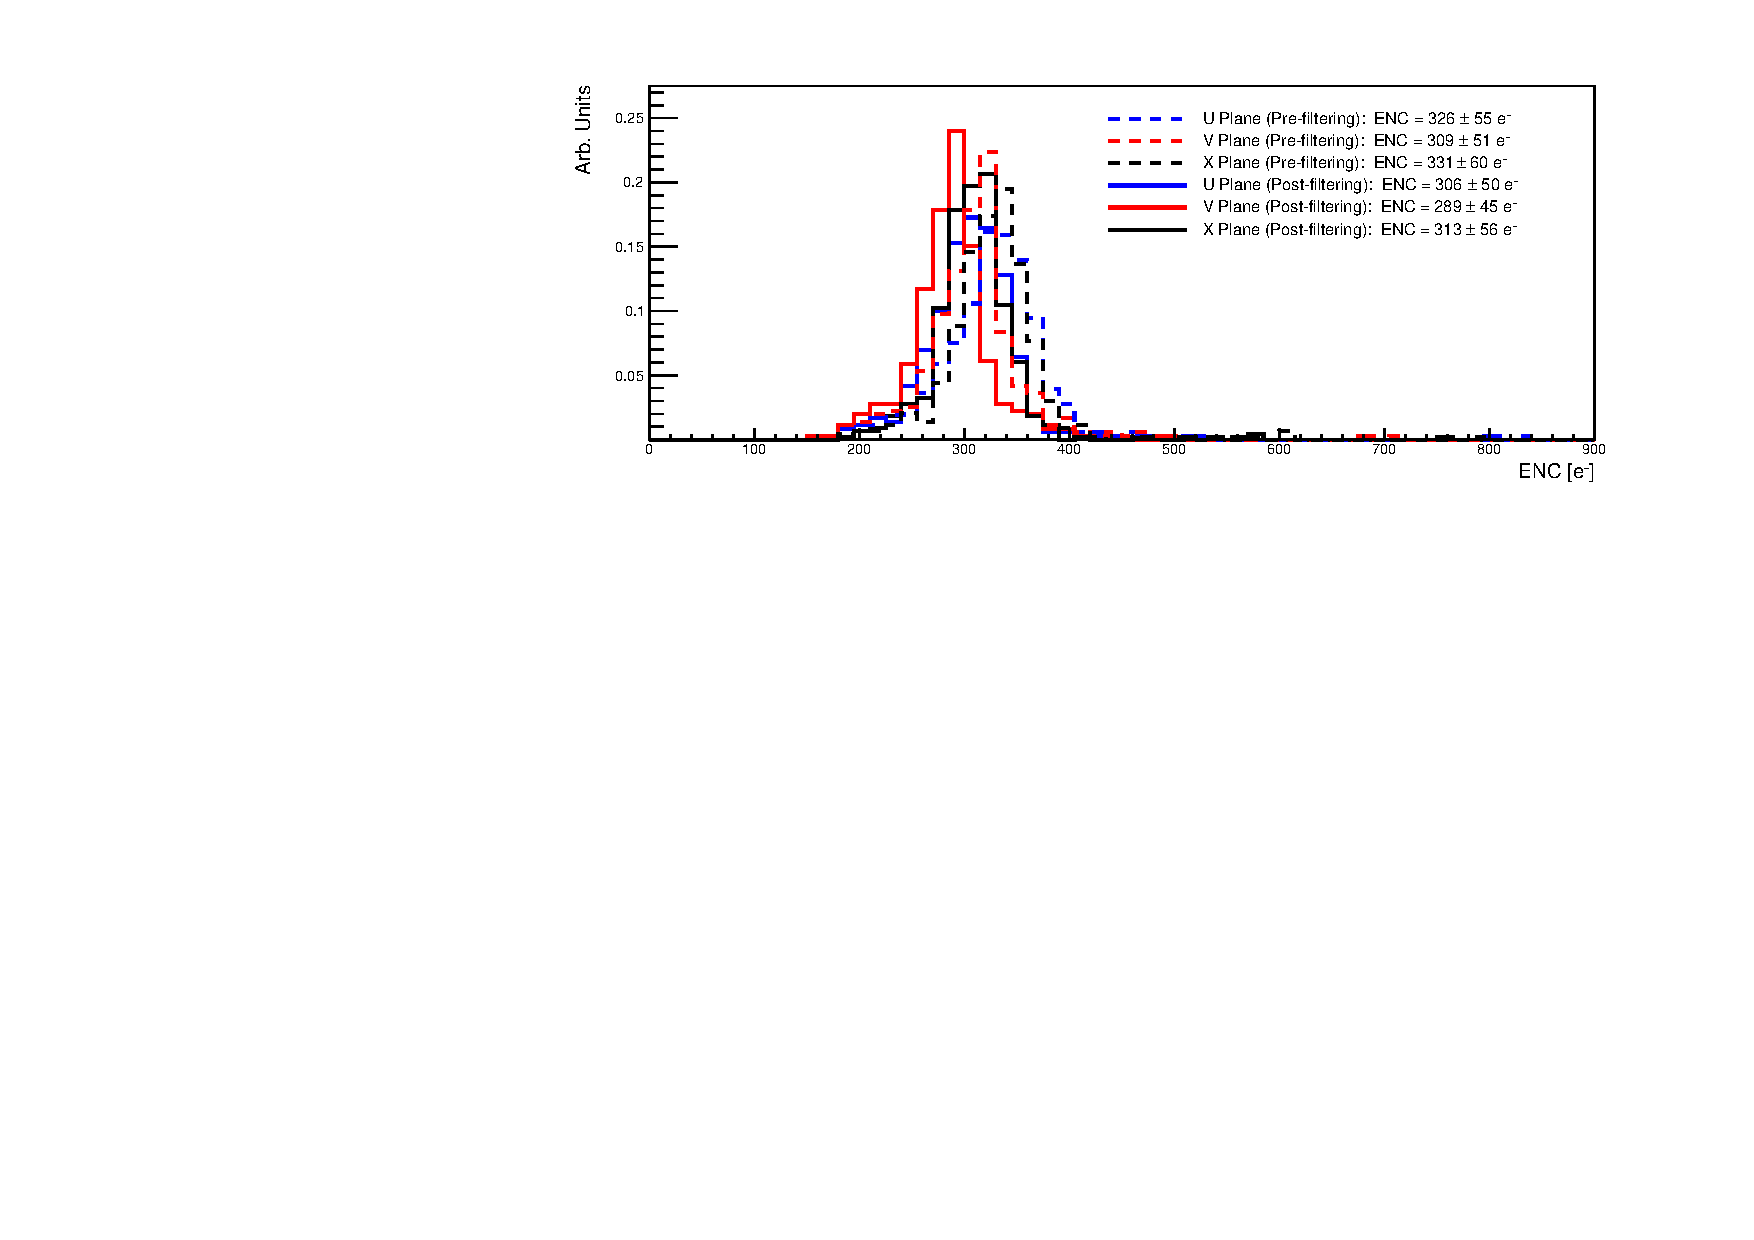
\includegraphics[width=0.99\linewidth]{sp-tpcelec-ENC-Combined-ICEBERG.pdf}
\end{dunefigure}


%%%%%%%%%%%%%%%%%%
\subsubsection{40\% APA at \dword{bnl}}
\label{sec:fdsp-tpcelec-qa-facilities-fortypercent}

One additional facility where the \dword{femb} prototypes can be connected to
an \dword{apa} inside a shielded environment is the \num{40}\,\% \dword{apa} 
test stand at \dword{bnl}. The \num{40}\,\% \dword{apa} at \dword{bnl} is a \SI{2.8}{m}~$\times$~\SI{1.0}{m} 
three-plane \dword{apa} with two layers of \num{576} wrapped ($U$ and $V$) wires 
and one layer of \num{448} straight ($X$) wires. It is read out by up to eight 
\dwords{femb} with the full length (\SI{7}{m}) \dword{pdsp} data and \dword{lv} power 
cables. The readout uses the full \dword{tpc} electronics 
system, including the \dword{ce} flange and \dword{wiec}, as shown in Figure~\ref{fig:tpcelec_40apa}. 
Detailed integration tests of the \dword{pdsp} \dword{ce} readout performance were done 
at the \num{40}\,\% \dword{apa}. During these tests the \dword{dune} grounding and shielding guidelines
were strictly followed.  This system was also used for initial studies of the \dword{cots} \dword{adc}
option that is described in Section~\ref{sec:fdsp-tpcelec-design-femb-alt-cots} and will
be used again for new \dword{femb} prototypes.

\begin{dunefigure}
[One side of the \num{40}\,\% APA with four FEMBs and the cold electronics flange]
{fig:tpcelec_40apa}
{Left: one side of the \num{40}\,\% \dword{apa} with four \dwords{femb}.  Right: the full \dword{ce} \fdth and flange.}
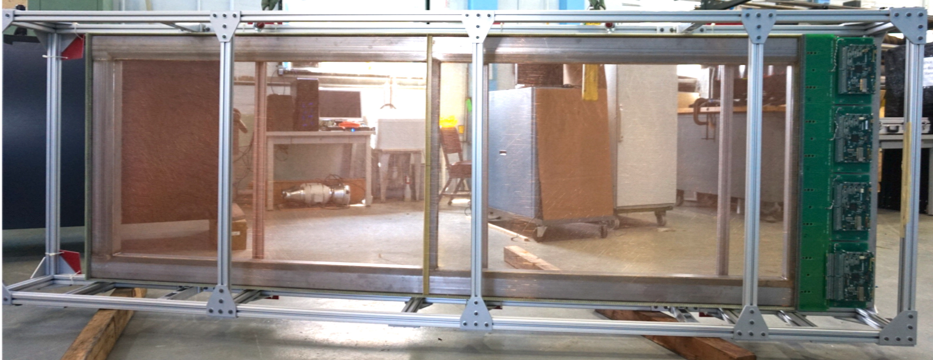
\includegraphics[width=0.72\linewidth]{sp-tpcelec-40-apa.png}
\hspace{3mm}
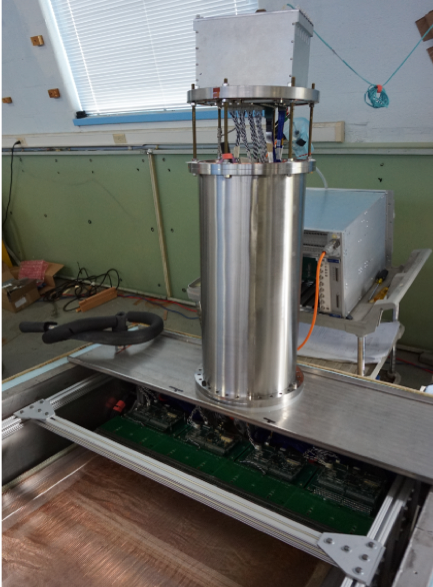
\includegraphics[width=0.2\linewidth]{sp-tpcelec-40-apa-ft.png}
\end{dunefigure}

Each of the three setups (\dword{apa} in the cold box at \dword{cern}, \dword{iceberg} \dword{tpc} at \dword{fnal},
and \num{40}\,\% \dword{apa} test stand at \dword{bnl}) that can be used for system tests has advantages
and disadvantages. Only the \dword{iceberg} \dword{tpc} can be used to 
perform measurements with tracks, but the \dword{apa} is 
much smaller than the \dword{dune} \dword{fd} \dword{apa} (which is also an advantage because it
allows us to determine the ultimate performance of the electronics because
the detector capacitance is reduced). The \dword{iceberg} \dword{tpc}
is for the moment the only setup compatible with the new \dword{pds}
design. Tests performed in the cold box at CERN and with the \num{40}\,\% \dword{apa} 
at \dword{bnl} are limited to noise measurements. These tests are not
performed at \dword{lar} temperature in the CERN setup. The advantage of
of the cold box at \dword{cern} and of tests performed in \dword{pdsp}
is that the \dword{apa} size is the one used in the \dword{dune} \dword{fd},
while the \dword{iceberg} detector is much smaller. We plan to continue
using all these setups for testing during the development of 
new \dwords{asic} and \dwords{femb} designs.

%%%%%%%%%%%%%%%%%%%%%%%%%%%%%%%%%%%
\subsection{Reliability Studies}
\label{sec:fdsp-tpcelec-qa-reliability}

The \dword{tpc} cold electronics system of the \dword{dune} \dword{sp} \dword{fd} must meet 
stringent requirements, including a very small number of failures ($<\num{1}$\% of the total number of
channels) for components installed 
on the detector inside the cryostat during the \dunelifetime of 
detector operation. Initial studies of the impact of dead channels indicate
that there is minimal impact on physics measurements even for a large ($\sim5$\%) number of 
channel failures randomly distributed in the detector, given the very high granularity of the \dword{tpc}. 
Further studies are ongoing to understand the impact of failures 
affecting groups of neighboring channels, which could arise from the failure of \dwords{asic} 
(16-64 channels) or \dwords{femb} (128 channels). Reliability must be incorporated in the 
design of all components, and a dedicated analysis of the physics impact of all 
possible failure modes, including a consideration of the number of readout channels
affected, is required before finalizing the design of all \dwords{asic}, printed circuit 
boards, cables, connectors, and their supports, all of which are housed inside the 
\dword{dune} \dword{fd} cryostat. 

A few \dword{hep} detectors have operated without intervention for a 
prolonged period, with few readout channel losses, in extreme 
conditions that are similar to those in the \dword{dune} \dword{fd} cryostats:
\begin{itemize}
\item The NA48/NA62 liquid krypton (LKr) calorimeter has 13,212 channels 
of JFET pre-amplifiers installed on the detector. It has been kept at LKr temperature 
since 1998. The total fraction of failed channels is $<$ 0.2\% in more than \num{20} years of operation.
\item The ATLAS \dword{lar} accordion electromagnetic barrel calorimeter has 
approximately 110,000 readout signal channels, with up to seven connections and different 
circuit boards populated with resistors and diodes inside the cryostat. This
calorimeter has been cold since 2004, for a total of \num{15} years of operation. So far, the
number of readout channels that have failed is approximately 0.02\% of the total channel count.
\item The ATLAS \dword{lar} hadronic endcap calorimeter has approximately 35,000 GaAs
pre-amplifers summed into 5,600 readout channels that are mounted on cold pre-amplifier
and summing boards. The ATLAS \dword{lar} hadronic endcap 
calorimeter cold electronics have been in cold since 2004, with
0.37\% of the channels failing during 15 years of operation. 
\end{itemize}
Since neither NA48/NA62 nor the ATLAS \dword{lar} hadronic endcap calorimeter
use \dword{cmos} electronics, the procedures used in the construction and \dword{qc} of \dwords{pcb} and 
for the selection and \dword{qc} of connectors and discrete components mounted
on the \dwords{pcb} represent the most relevant aspect for the \dword{dune} \dword{fd}.

In addition, FERMI/GLAST is an example of a joint project between \dword{nasa} and \dword{hep} groups 
with a minimum mission requirement of five years, and is on its way to achieving a 
stretch goal of ten years of operations in space. Although the requirements are somewhat 
different, examining and understanding the various strategies for a space 
flight project can inform the \dword{dune} project. 

A preliminary list of reliability topics to be studied for the \dword{tpc} electronics operated 
in \dword{lar} environment are:
\begin{itemize}
\item The custom \dwords{asic} proposed for use in \dword{dune} (\dword{larasic}, 
\dword{coldadc}, \dword{coldata}, and \dword{cryo}) incorporate design rules 
intended to minimize the hot-carrier effect~\cite{Li:CELAr,Hoff:2015hax}, 
which is recognized as the main failure mechanism for integrated circuits 
operating at \dword{lar} temperature.
\item For \dword{cots} components, accelerated lifetime testing, a methodology 
developed by \dword{nasa}~\cite{nasa_nepp} will be used to verify the expected
lifetime of operation at cryogenic temperatures. A \dword{cots} \dword{adc} has undergone
this procedure and has been qualified as a solution for the SBND experiment~\cite{Chen:2018zic}.
\item Printed circuit board assemblies are designed and fabricated to survive 
repeated immersions in \lntwo.
\item A study will be undertaken to give guidance on how much components (capacitors,
resistors, etc.) should be de-rated for power dissipation, operating voltage, etc.~in
order to achieve the desired reliability.
\item Similarly, connectors and cables, usually major sources of detector channel failures,
will require a separate study to identify optimal choices.
\item In addition to the \dword{qa} studies noted above, a very detailed
and formal set of \dword{qc} checks of the production pieces will be required in order to ensure
a reliable detector. The \dword{qc} plans for the \dword{tpc} electronics
detector components are discussed in Section~\ref{sec:fdsp-tpcelec-production-qc}.
\end{itemize}
The \dword{tpc} electronics consortium has formed a working group tasked with studying the reliability  
of these components, which is preparing recommendations for the choice of \dwords{asic}, 
the design of printed circuit boards, and testing procedures. This working group will review the 
segmentation of the cold electronics to understand which failures will most affect data taking, revisit recommendations for the \dword{asic} design, 
beyond those aimed at minimizing the hot-carrier effect, revisit the industry and 
\dword{nasa} standards for the design and fabrication of printed circuit boards, connectors, 
and cables, and recommend \dword{qc} procedures to be adopted during 
fabrication of the cold electronics components. The working group will also review
system aspects, to understand where it is desirable, necessary, and feasible to implement 
redundancy in the system in order to minimize data losses due to single component failures. 
